\contribution{Random Access Memory}
\shortcontributor{CS6230 : CAD for VLSI Project Report}
\shortcontribution{Overview}
\headnum{3}
\begin{paper}
\renewcommand*{\pagemark}{}

\section*{}
Memory access is the bottleneck in almost all of the vector operations. A multi-ported RAM with parallel read/writes coupled with a wide data bus is essential to profit from the vector accelerators' parallel processing capabilities.
\section*{Implimentation\sdot}
Vectors of EHRs were used to implement the RAM. CReg supplied by Bluespec limited the number of ports to 5. Assuming the smallest addressable unit is 1 byte (this is parameterized in the implementation), this limitation caused the throughput to be capped at 5 bytes per cycle. Another implementation of EHRs from {\color{RubineRed} https://web.mit.edu/6.375/install/bsvclib-2007-02-20\_19-10/EHR.bsv} removed this limitation, and the memory throughput is now only limited by the bus width. The ports followed the priority rules of EHRs. A wrapper was written to coordinate the ports and interface with the bus. To illustrate, if the bus requested only 1 byte, only one port would be active. On the other case, if the bus can transmit 64 bytes per cycle (512 bits) and requests for 512 bits, all 64 ports would be active.
\begin{figure}[H]
\centering
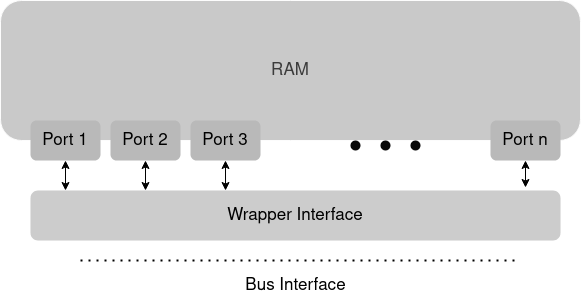
\includegraphics[width=7cm]{Images/Overview-Ram.png}
\caption{\content Ram wrapper interfaces bus to the ports.}
\end{figure}
\end{paper}